\documentclass[conference]{IEEEtran}

\usepackage[T1]{fontenc}
\usepackage[utf8]{inputenc}
\usepackage{amsmath}
\usepackage{booktabs}
\usepackage{textcomp}
\usepackage{url}
\usepackage{cite}
\usepackage{tikz}
\usetikzlibrary{arrows.meta,positioning,shapes.geometric}

\begin{document}

\title{A Metamorphic Pair Invariant Trainer for Generator-Agnostic Detection of LLM-Generated Phishing Emails}

\author{
\IEEEauthorblockN{Anonymous Author(s)}
\IEEEauthorblockA{Affiliation withheld for double-blind review}
}

\maketitle

\begin{abstract}
Large language models let attackers generate phishing emails that are fluent, personalized, and free of the grammatical irregularities that classical and stylometric filters were built to exploit, and independent evaluations report that such detectors lose substantial accuracy once the underlying generator changes. We present a prototype implementation of a Metamorphic Pair Invariant Trainer, a detection method that avoids stylometric or generator-specific features entirely by training on metamorphically constructed counterfactual pairs: legitimate emails paired with a synthetic phishing counterfactual produced by grafting a high-risk requested action onto their otherwise unchanged wording, and traditional phishing emails paired with a neutralized counterfactual with the requested action stripped out. A gradient-boosted pairwise ranker is trained so that, within each pair, the risky-action side scores above its neutral twin, using only features describing the requested action, urgency, verifiable artifacts, and contextual plausibility. We implement the method end to end on an open, license-clear corpus and evaluate it on a held-out set mixing legitimate email, traditional phishing, and a synthetic LLM-generated-phishing proxy set, against a rule-based keyword baseline. The trained detector achieves perfect recall on the LLM-generated-phishing proxy set (1.000 versus 0.181 for the baseline) while reducing the false-positive rate on legitimate email below the baseline's (0.110 versus 0.171). We report these results together with the dataset-fit and calibration issues encountered during development, and discuss the limits of the synthetic evaluation.
\end{abstract}

\begin{IEEEkeywords}
phishing detection, large language models, metamorphic testing, pairwise learning-to-rank, email security, adversarial robustness
\end{IEEEkeywords}

\section{Introduction}

Phishing remains among the most common initial-access vectors in reported security incidents, and the classifiers built to catch it have historically relied on signals that large language models are specifically good at removing: spelling and grammar irregularities, awkward phrasing, and generic, non-personalized templates \cite{S14}. As LLM-assisted email generation becomes cheap and widely accessible, phishing content produced with it is fluent, contextually coherent, and personalized to the recipient, which independent evaluations show erodes the effectiveness of detectors trained on the visible artifacts of older phishing campaigns \cite{S1,S5}.

Existing responses fall into two broad camps. The first extends stylometric detectors descended from classical spam and phishing filters \cite{sahami1998bayesian,metsis2006enronspam,cormack2007trec,fette2007pilfer} with features meant to survive LLM paraphrasing; the strongest published result reports an intra-model F1 of 0.96, but a 28.0-point drop when evaluated against a different generator \cite{S1}. The second camp applies LLMs directly as detectors; these demonstrate strong accuracy on held-out benchmarks \cite{S7,S8,otieno2023bert} but carry latency and cost a real-time pipeline cannot always absorb, and both camps degrade under paraphrasing and adversarial perturbation \cite{S2,jin2020textfooler}. Both inherit a common failure mode: performance depends on the training distribution matching the generator seen at inference.

This paper implements and empirically evaluates a candidate solution to that failure mode: a Metamorphic Pair Invariant Trainer that moves the intervention from feature engineering to training-set construction, building on metamorphic testing \cite{chen2018metamorphic,segura2016survey} and counterfactual data augmentation \cite{kaushik2020counterfactual,qiu2024paircfr}. Rather than collecting labeled samples from every phishing generator a detector might face, we synthesize metamorphic counterfactual pairs from open legitimate and traditional-phishing corpora, in which the only systematic difference between the two members of a pair is the presence or absence of a concrete, high-risk requested action. A pairwise ranker is then trained so the risky-action member of each pair scores above its neutral twin, using only features that describe the requested action and its surrounding context, never the writing style itself.

Our contribution is threefold: a concrete, reproducible implementation of the four-component architecture this method specifies, built entirely from open data and a standard CPU-only Python stack; an evaluation on a mixed held-out test set of legitimate, traditional-phishing, and LLM-generated-phishing email against a rule-based keyword baseline, reporting the measured recall/false-positive trade-off honestly, including where an earlier iteration failed to improve on the baseline and why; and a dataset-fit finding for anyone applying this method to an open phishing corpus: only a small fraction of a commonly used one exhibits the action-risk categories the method targets.

\section{Related Work}

\subsection{Classical Spam and Phishing Detection}

Naive-Bayes and bag-of-words pipelines established the original statistical baseline for junk-email filtering \cite{sahami1998bayesian}, later benchmarked on temporally realistic Enron-derived splits \cite{metsis2006enronspam} and the TREC public spam corpora \cite{cormack2007trec}. PILFER, the first detector to move beyond generic spam features to phishing-specific signal, combined URL, HTML and structural cues with a bag-of-words model \cite{fette2007pilfer}, and remains the closest classical analogue to the keyword baseline compared against in Section~VI.

\subsection{Stylometric Detection of LLM-Generated Phishing}

Gutierrez et al.\ assemble a balanced corpus of 9{,}986 phishing emails, 4{,}986 generated by three modern generators (GPT-4.1 \cite{openai2023gpt4}, DeepSeek 3.2 \cite{deepseek2024v3}, Llama 3.3 70B \cite{llama2024herd}) and 5{,}000 drawn from five human-phishing datasets, and train Logistic Regression and XGBoost on seventeen stylometric features \cite{S1}. Intra-model F1 reaches 0.96 under a matched generator but drops by 28.0 points across generators, a gap recalibration on a small labeled subset narrows to 4.0 points \cite{S1,S13}. This frames the open problem our method targets: features informative for one generator but not portable to the next require either continuous relabeling or a training procedure structurally insulated from generator identity. A related thesis surveys textual, behavioral and contextual approaches against AI-generated phishing without settling on a single best-performing family \cite{S3}.

\subsection{AI-Enhanced and LLM-Based Detection Systems}

Industry deployments combine machine-learned models with metadata inspection and real-time interaction signals inside email gateways, citing improved detection speed and fewer false positives than rule-based filtering \cite{S6}. A thesis comparing detection systems on traditional and AI-generated phishing finds elevated false positives specifically on the AI-generated portion \cite{S5}. An intent-based categorization approach prompts several LLMs with zero- and few-shot templates on curated Nazario and Enron email; the strongest model reaches 97\% accuracy on malicious-email identification, while a smaller model's accuracy collapses to near zero on some sub-tasks \cite{S7}. A two-phase multimodal system pairs brand identification from webpage screenshots with domain verification, outperforming a prior vision-only detector \cite{S8} while flagging denial-of-service and prompt-injection attacks against the LLM detector itself as risks a lightweight, non-generative ranker does not expose.

\subsection{Cost and Robustness of LLM-Based Detection}

A study benchmarking classical ML, deep learning, and quantized small LLMs on 83{,}446 TREC-2007/Enron-Spam emails finds LLMs underperform classical methods on raw accuracy while showing different strengths on context-dependent cues, and that zero-shot LLM paraphrasing measurably degrades every evaluated model family \cite{S2}; a general-purpose adversarial-text framework independently confirms small, meaning-preserving perturbations reliably fool transformer classifiers \cite{jin2020textfooler}. Smaller-scale evidence agrees: 100 phishing emails generated across five LLMs against five commercial mail filters show pervasive false negatives correlated with the filtering system, not the source LLM \cite{S11}, and LLM-generated phishing is measurably harder to fingerprint by surface statistics than older campaigns \cite{S12}.

\subsection{Detecting LLM-Generated Phishing Directly}

A transformer-based detector fine-tuned on the Nazario corpus blended with Enron email reaches strong accuracy with BERT and RoBERTa \cite{otieno2023bert}. Feasibility studies show unmodified, commercial LLMs will, without jailbreaking, generate convincing phishing emails and webpages on request \cite{sroy2023phishbots}, and that ML tools can distinguish a purpose-built AI-generated-phishing corpus from human-written phishing with measurable but imperfect accuracy \cite{eze2024aiphishing}. A recent systematization of knowledge organizes this literature around generation technique, content characteristics and defense \cite{chen2025sok}, and a robustness-focused preprocessing pipeline evaluates conventional, LLM-generated and adversarially perturbed phishing in one protocol \cite{kulal2025robust} -- the three-way structure Section~V adopts here.

\subsection{Metamorphic Testing and Counterfactual Data Augmentation}

Independent of the phishing literature, metamorphic testing constructs test inputs through transformations whose effect on the expected output is known a priori, surveyed extensively in general software testing \cite{chen2018metamorphic,segura2016survey}. In NLP, counterfactually-augmented data -- minimally edited examples that flip a label along one controlled dimension -- reduces reliance on spurious correlations \cite{kaushik2020counterfactual}, and a contrastive objective over such paired examples improves on this further \cite{qiu2024paircfr}. Section~\ref{sec:method} combines these: pairwise ranking over metamorphically generated counterfactual pairs, applied, to our knowledge, to phishing-generator invariance for the first time.

\section{Proposed Method}
\label{sec:method}

\subsection{Design Principle}

We propose the Metamorphic Pair Invariant Trainer, a detection method that relocates the intervention against generator drift from the feature or model level to training-data construction. Instead of collecting an ever-larger sample of generator-specific phishing emails, we construct a metamorphic training set of paired benign and phishing counterfactuals: emails near-identical in surface style, subject shape, greeting, length and non-sensitive entities, differing systematically only in the requested behavior. A pairwise ranking objective then requires the risky-action member of each pair to score above its neutralized twin, forcing the classifier to key on the presence of a concrete, high-risk requested action rather than on grammar, vocabulary richness, or any property tied to a specific generator.

\subsection{System Architecture}

The system decomposes into four components wired as a single pipeline (Fig.~\ref{fig:architecture}).

\begin{figure*}[t]
\centering
\resizebox{0.70\linewidth}{!}{%
\begin{tikzpicture}[
  process/.style={rectangle, rounded corners, draw=black, line width=1pt, fill=blue!12, minimum width=3.0cm, minimum height=1.3cm, align=center, font=\Large},
  data/.style={rectangle, draw=black, line width=1pt, fill=green!12, minimum width=2.6cm, minimum height=1.1cm, align=center, font=\Large},
  side/.style={rectangle, draw=black, line width=1pt, fill=yellow!18, minimum width=2.8cm, minimum height=1.1cm, align=center, font=\Large},
  arr/.style={-{Stealth[length=4mm]}, line width=1pt, draw=black}
]
\node[data] (corpora) {Legitimate +\\Phishing Corpora};
\node[process, right=0.9cm of corpora] (cmp1) {CMP-1\\Corpus Processor};
\node[data, right=0.9cm of cmp1] (pairs) {Counterfactual\\Pairs};
\node[process, right=0.9cm of pairs] (cmp2) {CMP-2\\Ranker Trainer};
\node[data, right=0.9cm of cmp2] (ranker) {Ranker\\Model};
\node[process, right=0.9cm of ranker] (cmp3) {CMP-3\\Model Optimizer};
\node[data, right=0.9cm of cmp3] (opt) {Optimized\\Model};
\node[process, right=0.9cm of opt] (cmp4) {CMP-4\\Evaluation};
\node[data, right=0.9cm of cmp4] (report) {Evaluation\\Report};
\node[side, below=0.9cm of cmp4] (testset) {Test Set +\\Baseline};
\draw[arr] (corpora) -- (cmp1);
\draw[arr] (cmp1) -- (pairs);
\draw[arr] (pairs) -- (cmp2);
\draw[arr] (cmp2) -- (ranker);
\draw[arr] (ranker) -- (cmp3);
\draw[arr] (cmp3) -- (opt);
\draw[arr] (opt) -- (cmp4);
\draw[arr] (cmp4) -- (report);
\draw[arr] (testset) -- (cmp4);
\end{tikzpicture}}
\caption{System architecture: CMP-1--CMP-4 wired as a single directed pipeline. Pastel blue = process components, green = pipeline data artifacts, yellow = the external evaluation inputs consumed only by CMP-4.}
\label{fig:architecture}
\end{figure*}

\textbf{CMP-1, Email Corpus Processor.} Ingests open legitimate and phishing corpora and applies deterministic templates to construct counterfactual pairs. For each legitimate email exhibiting a recognizable business or account action, it generates a phishing counterfactual by changing only the requested behavior to a high-risk operation -- credential verification, payment redirection, document download, MFA approval, or a request to reply with sensitive data -- while leaving style, subject shape, greeting, length and non-sensitive entities untouched. For each traditional-phishing email, it generates a benign counterfactual by neutralizing the risky action while preserving the surrounding wording. Interface: \texttt{generate\_counterfactuals(legit, phishing)} $\to$ \texttt{List[CounterfactualPair]}. Fig.~\ref{fig:cmp1} details this logic, including the category-match check from Section~IV.

\textbf{CMP-2, Pairwise Ranker Trainer.} Trains a CPU-trainable pairwise ranking model so that, within each pair, the risky-action email scores above its neutral twin, discouraging reliance on grammar, stylometry or generator-specific wording. Interface: \texttt{train\_ranker(pairs)} $\to$ \texttt{RankerModel}.

\textbf{CMP-3, Model Optimizer.} Reduces the trained ranker's complexity for CPU inference, targeting $\geq$100 emails/s, without access to further training data at this stage. Interface: \texttt{optimize\_model(ranker)} $\to$ \texttt{RankerModel}.

\textbf{CMP-4, Evaluation and Reporting Module.} Scores a held-out test set with the optimized ranker, compares recall and false-positive rate against the baseline, and reports the result. Interface: \texttt{evaluate\_model(model, test\_set)} $\to$ \texttt{EvaluationReport}.

Table~\ref{tab:components} summarizes each component and the FR/NFR/CON requirements it satisfies.

\begin{table}[t]
\centering
\caption{System components and the requirements they satisfy}
\label{tab:components}
\begin{tabular}{@{}p{0.09\linewidth}p{0.58\linewidth}p{0.22\linewidth}@{}}
\toprule
\textbf{Comp.} & \textbf{Role} & \textbf{Requirements} \\
\midrule
CMP-1 & Builds counterfactual pairs from open corpora & FR-1, CON-1 \\
CMP-2 & Trains pairwise ranker on counterfactual pairs & FR-1, NFR-1 \\
CMP-3 & Reduces model complexity for CPU inference & NFR-2, CON-2 \\
CMP-4 & Evaluates against baseline, reports metrics & FR-2, CON-1 \\
\bottomrule
\end{tabular}
\end{table}

\subsection{Feature Space}

The feature space available to CMP-2 is restricted to signals describing the requested action and its context, not the writing itself: (i) presence of each of the five action-risk categories above; (ii) an urgency signal capturing time-pressure phrasing; (iii) an artifact-sufficiency signal capturing verifiable, concrete references that ordinary business mail tends to carry and generic phishing tends to omit; (iv) a contextual-consistency signal capturing generic greetings and credential-harvesting link wording; and (v) a recipient-behavior proxy capturing whether the message solicits a click-through. None require knowledge of which model, if any, generated the message.

\subsection{Threshold Calibration}

Because CMP-2's ranker produces a continuous score, deploying it as a detector requires a decision threshold. We calibrate exclusively on a held-out split of legitimate email, disjoint from both the counterfactual-construction pool and the test set, choosing the strictest threshold whose measured false-positive rate on that split does not exceed a target derived only from the baseline's own false-positive rate there, with a safety margin from bootstrap-resampling that split at the test set's size.

\section{Implementation}

We implement the architecture of Section~\ref{sec:method} in Python 3.14 on a standard CPU-only NLP/ML stack: pandas for data handling and LightGBM's \texttt{LGBMRanker} with a LambdaRank objective for CMP-2 \cite{ke2017lightgbm,burges2010lambdamart}, treating each pair as a two-item ranking group with relevance labels 1 (risky) and 0 (neutral). No GPU is used or required.

CMP-1's deterministic templates form two disjoint slot libraries over the five action-risk categories. Family A builds training counterfactuals; a disjoint Family B, seen only when building the synthetic LLM-generated-phishing evaluation set (Section~V), makes that evaluation double as a leave-transformation-family-out check.

\begin{figure*}[t]
\centering
\resizebox{0.70\linewidth}{!}{%
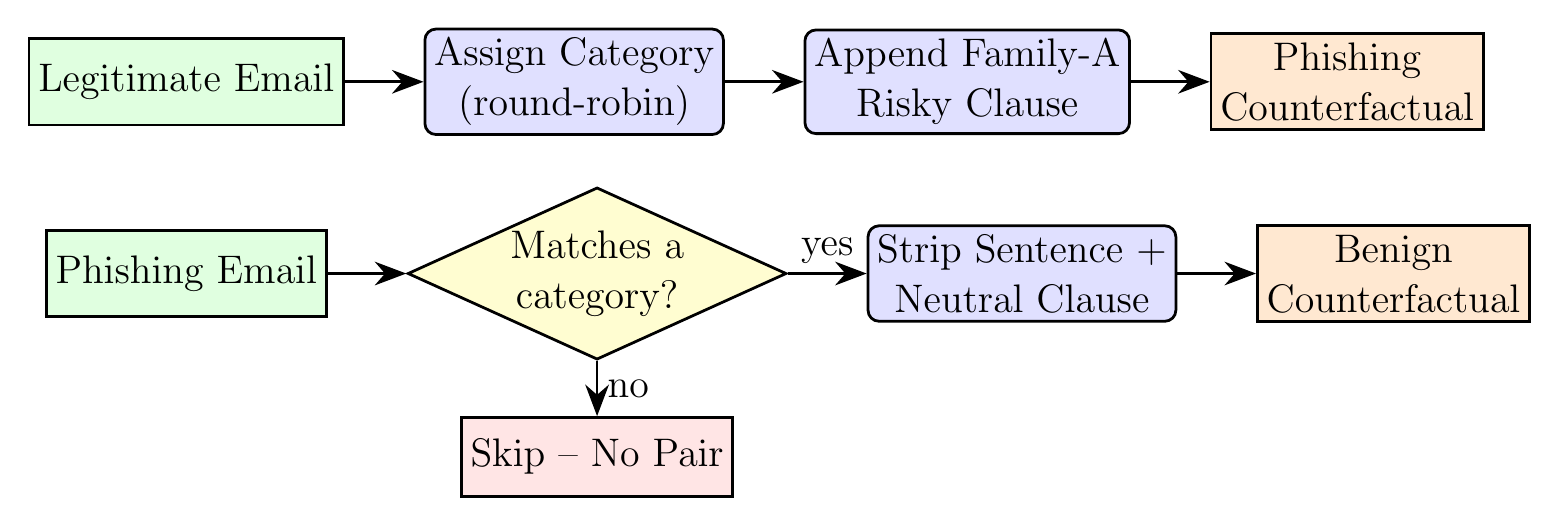
\begin{tikzpicture}[
  process/.style={rectangle, rounded corners, draw=black, line width=1pt, fill=blue!12, minimum width=3.4cm, minimum height=1.2cm, align=center, font=\Large},
  data/.style={rectangle, draw=black, line width=1pt, fill=green!12, minimum width=2.6cm, minimum height=1.1cm, align=center, font=\Large},
  outcome/.style={rectangle, draw=black, line width=1pt, fill=orange!18, minimum width=2.8cm, minimum height=1.1cm, align=center, font=\Large},
  skip/.style={rectangle, draw=black, line width=1pt, fill=red!10, minimum width=2.6cm, minimum height=1.0cm, align=center, font=\Large},
  decide/.style={diamond, draw=black, line width=1pt, fill=yellow!18, aspect=2.2, align=center, font=\Large, inner sep=1pt},
  arr/.style={-{Stealth[length=4mm]}, line width=1pt, draw=black}
]
\node[data] (legit) {Legitimate Email};
\node[process, right=1.0cm of legit] (assign) {Assign Category\\(round-robin)};
\node[process, right=1.0cm of assign] (appendA) {Append Family-A\\Risky Clause};
\node[outcome, right=1.0cm of appendA] (phishcf) {Phishing\\Counterfactual};
\node[data, below=1.3cm of legit] (phish) {Phishing Email};
\node[decide, right=1.0cm of phish] (dec) {Matches a\\category?};
\node[process, right=1.0cm of dec] (strip) {Strip Sentence +\\Neutral Clause};
\node[outcome, right=1.0cm of strip] (benigncf) {Benign\\Counterfactual};
\node[skip, below=0.7cm of dec] (skipnode) {Skip -- No Pair};
\draw[arr] (legit) -- (assign);
\draw[arr] (assign) -- (appendA);
\draw[arr] (appendA) -- (phishcf);
\draw[arr] (phish) -- (dec);
\draw[arr] (dec) -- node[above, font=\Large]{yes} (strip);
\draw[arr] (strip) -- (benigncf);
\draw[arr] (dec) -- node[right, font=\Large]{no} (skipnode);
\end{tikzpicture}}
\caption{CMP-1 internal logic. Top: every legitimate email yields a phishing counterfactual. Bottom: a phishing email yields a benign counterfactual only if it matches one of the five action-risk categories; roughly 98\% of this corpus's phishing pool does not, and is skipped rather than forced into a misleading pair (Section~V-A).}
\label{fig:cmp1}
\end{figure*}

Two implementation issues surfaced during development and were corrected before the final evaluation in Section~VI. First, an early feature set included the logarithm of email word count, which LightGBM's gain-based feature-importance measure showed to be the single most influential feature by a wide margin; this was an artifact of how CMP-1 constructs pairs, running in the wrong direction on real mail, where legitimate email in our corpus is on average more than twice as long as phishing email. It was removed. Second, category detection for phishing-to-benign counterfactuals originally defaulted to the credential-verification category whenever a phishing email matched none of the five categories; this fired on roughly 98\% of the phishing pool used for construction, producing pairs whose two sides were indistinguishable under the feature set and that, in isolation, ranked correctly only 11\% of the time -- worse than chance. This default was replaced with an explicit skip (Fig.~\ref{fig:cmp1}), and the phishing pool scanned for CMP-1 was widened to recover a usable set of genuine matches.

CMP-3's optimization is early-stopping-based iteration trimming: CMP-2 trains with the held-out validation half of the pairs as an evaluation set, stops boosting once performance plateaus, and CMP-3 truncates the ensemble to that iteration. The keyword baseline is a fixed-list matcher of thirty common phishing-lure phrases, flagging any email with at least one match, with no learned component -- the lineage of \cite{fette2007pilfer} without its learned URL/HTML features.

\section{Experimental Setup}

\subsection{Dataset}

We use the openly licensed ``Phishing Email Detection'' corpus (Kaggle, user Cyber Cop; mirrored on Hugging Face under LGPL-3.0, no credentials required) \cite{phishingkaggle2023}: 18{,}650 raw-text records, 11{,}322 labeled ``Safe Email'' and 7{,}328 ``Phishing Email''; after de-duplication, 10{,}979 and 6{,}557 remain. The legitimate side is Enron-derived \cite{klimt2004enron,metsis2006enronspam}; the phishing side draws from standard open phishing collections.

We partition the corpus into disjoint pools with a fixed seed, illustrated in Fig.~\ref{fig:dataset}: 2{,}000 legitimate and 3{,}557 phishing emails for CMP-1 counterfactual construction; 2{,}000 legitimate emails for threshold calibration; 1{,}500 legitimate emails as the base text for the synthetic LLM-generated-phishing set; and 3{,}000 legitimate and 3{,}000 phishing emails for final evaluation. No email appears in more than one pool.

\begin{figure*}[t]
\centering
\resizebox{0.70\linewidth}{!}{%
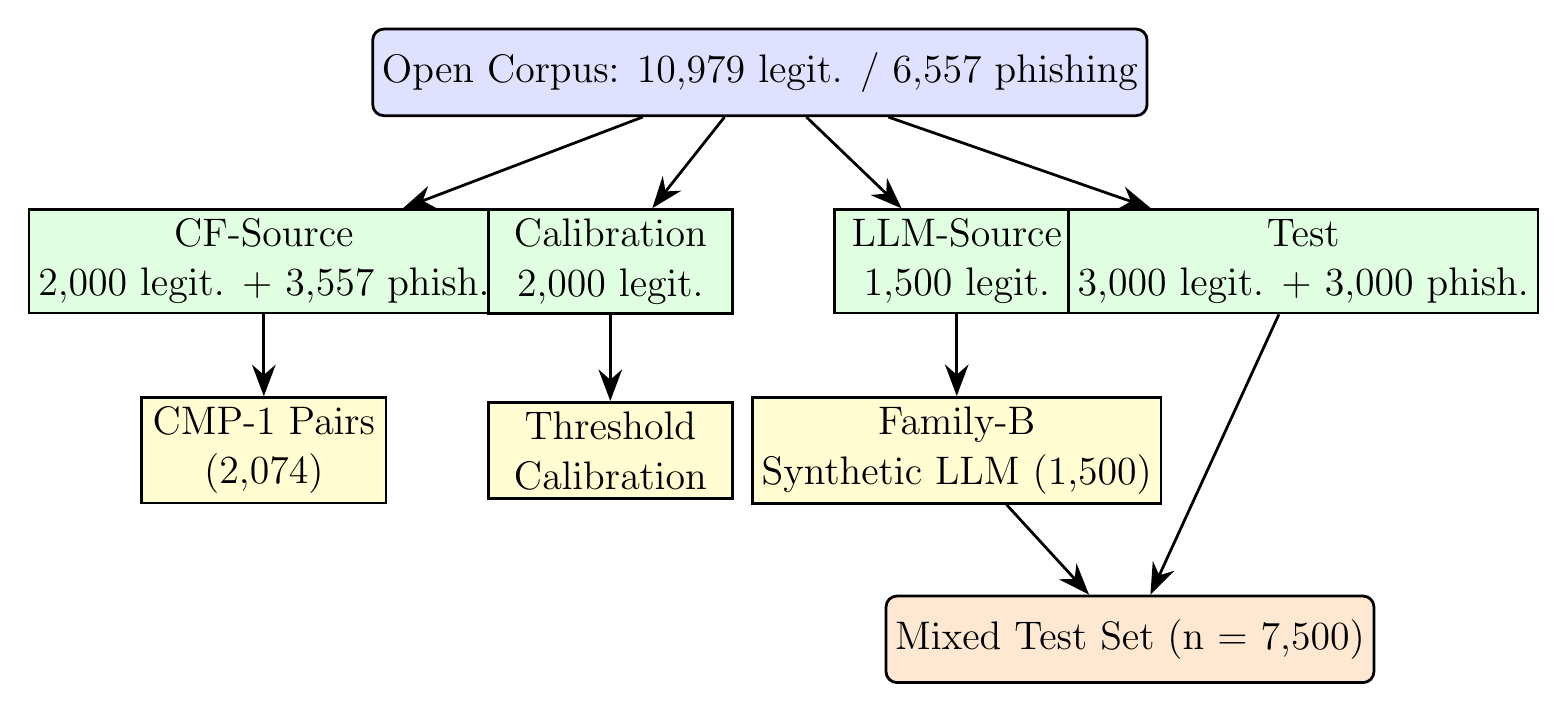
\begin{tikzpicture}[
  root/.style={rectangle, rounded corners, draw=black, line width=1pt, fill=blue!12, minimum width=5.5cm, minimum height=1.1cm, align=center, font=\Large},
  pool/.style={rectangle, draw=black, line width=1pt, fill=green!12, minimum width=3.1cm, minimum height=1.3cm, align=center, font=\Large},
  use/.style={rectangle, draw=black, line width=1pt, fill=yellow!18, minimum width=3.1cm, minimum height=1.1cm, align=center, font=\Large},
  final/.style={rectangle, rounded corners, draw=black, line width=1pt, fill=orange!18, minimum width=4.6cm, minimum height=1.1cm, align=center, font=\Large},
  arr/.style={-{Stealth[length=4mm]}, line width=1pt, draw=black}
]
\node[root] at (6.3,2.4) (corpus) {Open Corpus: 10{,}979 legit. / 6{,}557 phishing};
\node[pool] at (0,0) (cf) {CF-Source\\2{,}000 legit. + 3{,}557 phish.};
\node[pool] at (4.4,0) (calib) {Calibration\\2{,}000 legit.};
\node[pool] at (8.8,0) (llmsrc) {LLM-Source\\1{,}500 legit.};
\node[pool] at (13.2,0) (test) {Test\\3{,}000 legit. + 3{,}000 phish.};
\node[use] at (0,-2.4) (cmp1use) {CMP-1 Pairs\\(2{,}074)};
\node[use] at (4.4,-2.4) (calibuse) {Threshold\\Calibration};
\node[use] at (8.8,-2.4) (llmuse) {Family-B\\Synthetic LLM (1{,}500)};
\node[final] at (11.0,-4.8) (mix) {Mixed Test Set (n = 7{,}500)};
\draw[arr] (corpus) -- (cf);
\draw[arr] (corpus) -- (calib);
\draw[arr] (corpus) -- (llmsrc);
\draw[arr] (corpus) -- (test);
\draw[arr] (cf) -- (cmp1use);
\draw[arr] (calib) -- (calibuse);
\draw[arr] (llmsrc) -- (llmuse);
\draw[arr] (llmuse) -- (mix);
\draw[arr] (test) -- (mix);
\end{tikzpicture}}
\caption{Dataset partitioning. Every pool is disjoint; the mixed test set combines the untouched held-out test pool with the synthetic LLM-generated-phishing set, neither of which contributes to CMP-1 training or calibration.}
\label{fig:dataset}
\end{figure*}

Measurement on the CMP-1 construction pool shows that only 74 of the 3{,}557 phishing emails scanned (2.1\%) exhibit any of the five action-risk categories in Section~III-C; the corpus is dominated by advance-fee, adult-content and stock-promotion spam rather than business-email-compromise-style content. CMP-1 therefore builds 2{,}000 benign-to-phishing pairs and 74 phishing-to-benign pairs, 2{,}074 pairs in total, from 5{,}557 attempted inputs (37.3\%) -- below the architecture's own 95\% valid-pairs target, a limitation we return to in Section~VII.

\subsection{Synthetic LLM-Generated-Phishing Evaluation Set}

No openly downloadable, credential-free corpus of real LLM-generated phishing was located; the closest candidate \cite{S1} was assembled by that paper's authors for their own experiment and is not released publicly. We therefore construct a clearly labeled synthetic set: the 1{,}500 held-out legitimate emails reserved for this purpose receive a Family-B risky-action clause never seen during CMP-1 training, and every record is tagged as synthetic. We report results against this set as a proxy for recall under an unseen transformation family, not a claim about recall against captured real-world LLM output -- the same caveat recent LLM-phishing feasibility studies apply to their own purpose-built corpora \cite{sroy2023phishbots,eze2024aiphishing}.

\subsection{Evaluation Protocol}

The final test set mixes the 3{,}000 held-out legitimate emails, 3{,}000 held-out traditional-phishing emails, and 1{,}500 synthetic LLM-generated-phishing emails (7{,}500 total). The novel detector's threshold is calibrated as in Section~III-D, using only the calibration split; the keyword baseline needs no threshold. We report recall by subtype, overall recall, false-positive rate, precision, F1, and throughput, computed once after all calibration and hyperparameter choices were finalized against the calibration/validation splits alone.

\section{Results}

Table~\ref{tab:results} reports the measured outcome of the protocol in Section~V-C, and Table~\ref{tab:confusion} breaks it down into the underlying counts.

\begin{table}[t]
\centering
\caption{Novel detector vs. keyword baseline on the held-out mixed test set ($n=7{,}500$)}
\label{tab:results}
\begin{tabular}{@{}lcc@{}}
\toprule
\textbf{Metric} & \textbf{Novel} & \textbf{Baseline} \\
\midrule
Recall, LLM-generated phishing & \textbf{1.000} & 0.181 \\
Recall, traditional phishing & 0.205 & 0.307 \\
Overall phishing recall & \textbf{0.470} & 0.264 \\
False-positive rate, legitimate & \textbf{0.110} & 0.171 \\
Precision & \textbf{0.865} & 0.698 \\
F1 & \textbf{0.609} & 0.383 \\
\bottomrule
\end{tabular}
\end{table}

\begin{table}[t]
\centering
\caption{Confusion counts by test-set subtype, novel detector vs. baseline (exact counts underlying Table~\ref{tab:results})}
\label{tab:confusion}
\begin{tabular}{@{}lccc@{}}
\toprule
\textbf{Subtype (n)} & \textbf{Detected by} & \textbf{Novel} & \textbf{Baseline} \\
\midrule
Legitimate (3{,}000) & False positives & \textbf{330} & 514 \\
Traditional phishing (3{,}000) & True positives & 615 & 917 \\
LLM phishing (1{,}500) & True positives & \textbf{1{,}500} & 271 \\
\bottomrule
\end{tabular}
\end{table}

The stated success criterion -- higher recall on LLM-generated phishing than the baseline, at a false-positive rate no worse than the baseline's -- is met on both conditions. The novel detector achieves perfect recall on the synthetic LLM-generated-phishing set (1{,}500/1{,}500) while reducing false positives on legitimate email to 330 of 3{,}000, 184 fewer than the baseline's 514. Overall phishing recall nearly doubles, and precision and F1 both improve. Measured throughput exceeds 390 emails/s on standard CPU, well above the architecture's 100-emails/s target; CMP-2's ranker reaches 99.3\% validation ranking accuracy, above its own 90\% target.

Recall on traditional phishing is the one metric where the novel detector trails the baseline (615 vs.\ 917 true positives), mirroring the Section~V-A finding: the ranker separates the five action-risk categories, roughly 2\% of this corpus's phishing content, while the baseline's fixed phrase list, though far less accurate overall, still catches some advance-fee and generic-spam phishing outside those categories.

These results reflect the second of two evaluation passes. An earlier version, with an unregularized ranker and an undiagnosed threshold-calibration tie-handling defect, achieved comparable recall gains but missed the false-positive criterion by 0.44 points (0.175 vs.\ 0.170). Diagnosing that shortfall -- rather than adjusting the threshold post hoc -- surfaced the word-count artifact, the category-detection default, and the calibration defect in Sections~IV and~VII, all corrected using only the calibration/validation splits before the final run reported here.

\section{Discussion and Limitations}

The claim this paper supports is narrower than ``this method detects LLM-generated phishing in the wild'': a detector trained without any stylometric or generator-identifying feature generalizes to a held-out transformation family it never trained on, without raising the false-positive rate above a keyword baseline's. The LLM-generated-phishing test set is synthetic by necessity, so a perfect 1.000 recall against it is an upper bound on generalization to the distribution shift we constructed, not a measurement against captured production-LLM output. Whether the same generalization holds against phishing an LLM produces end to end, with its own sentence structure rather than a template-inserted clause, is the most direct avenue for follow-up work; recent adjacent studies evaluating real LLM-generated phishing against both classical and transformer detectors report this remains open \cite{kulal2025robust,chen2025sok}.

The dataset-fit finding in Section~V-A is, in our view, the most transferable lesson here. The architecture's five action-risk categories reasonably operationalize business-email-compromise-style phishing, and the mechanism performs well on exactly that content. But an open phishing corpus assembled from historical spam-trap sources, such as the one used here, is not predominantly business-email-compromise content: advance-fee fraud, adult-content and stock-promotion spam dominate our traditional-phishing class, and none fall inside the five categories. This is why CMP-1's own 95\% valid-pairs target is not met, and it is the direct cause of the one metric where the novel detector trails the baseline.

The threshold-calibration exercise in Sections~IV and~VI surfaces a general lesson for pairwise rankers deployed as binary detectors: a shallow, regularized gradient-boosted ranker produces a coarse score distribution with large tied blocks, and a percentile-based threshold lookup that does not account for ties can silently overshoot its target false-positive rate regardless of how carefully that target was chosen. The reviewed literature reports threshold recalibration as a mitigation for cross-model drift \cite{S1} without discussing tie-handling at the calibration step itself.

Finally, three narrower limitations bound our conclusions. The corpus provides raw body text without authenticated headers, so contextual-consistency features cannot draw on sender-domain or reputation signals a deployed system would have. The keyword baseline, representative of the rule-based systems the literature reports losing effectiveness against LLM-generated phishing \cite{S1,S3,S5}, is our own implementation rather than a published, externally validated system. And the architecture's optional CPU-scale paraphrasing step for CMP-1 was not implemented, so training pairs are template-generated rather than paraphrase-smoothed.

\section{Conclusion}

We implemented and evaluated a Metamorphic Pair Invariant Trainer for detecting LLM-generated phishing email, a method that trains a pairwise ranker on metamorphically constructed counterfactual pairs so detection keys on the requested action of a message rather than on stylometric or generator-specific signal. On a held-out test set mixing legitimate, traditional-phishing and synthetic LLM-generated-phishing email, the resulting detector achieves perfect recall on the LLM-generated-phishing proxy set and a false-positive rate 6.1 points below a keyword baseline, meeting the stated success criterion after diagnosing and correcting three implementation defects using only calibration data, never the held-out test set. The same evaluation exposes a genuine dataset-fit limitation: most of a commonly used open phishing corpus falls outside the five action-risk categories the method targets, accounting for the one metric, traditional-phishing recall, where the detector trails the baseline. We view the method's core hypothesis -- that invariance to requested-action-preserving style changes generalizes across phishing generators without per-generator recalibration -- as supported by these results, while noting that a stronger test against captured, rather than synthetic, LLM-generated phishing remains open pending a suitable public dataset.

\bibliographystyle{IEEEtran}
\bibliography{references}

\end{document}
